\documentclass[        
    a4paper,          % Tamanho da folha A4
    12pt,             % Tamanho da fonte 12pt
    chapter=TITLE,    % Todos os capitulos devem ter caixa alta
    section=Title,    % Todas as secoes devem ter caixa alta somente na primeira letra
    subsection=Title, % Todas as subsecoes devem ter caixa alta somente na primeira letra
    oneside,          % Usada para impressao em apenas uma face do papel
    english,          % Hifenizacoes em ingles
    spanish,          % Hifenizacoes em espanhol
    brazil,           % Ultimo idioma eh o idioma padrao do documento
    %fleqn             % Comente esta linha se quiser centralizar as equacoes. Comente também a linha 65 abaixo
]{abntex2}

% Importações de pacotes
\usepackage[utf8]{inputenc}                         % Acentuação direta
\usepackage[T1]{fontenc}                            % Codificação da fonte em 8 bits
\usepackage{graphicx}                               % Inserir figuras
\usepackage{amsfonts, amssymb, amsmath}             % Fonte e símbolos matemáticos
\usepackage{booktabs}                               % Comandos para tabelas
\usepackage{verbatim}                               % Texto é interpretado como escrito no documento
\usepackage{multirow, array}                        % Múltiplas linhas e colunas em tabelas
\usepackage{indentfirst}                            % Endenta o primeiro parágrafo de cada seção.
\usepackage{listings}                               % Utilizar codigo fonte no documento
\usepackage{xcolor}
\usepackage{microtype}                              % Para melhorias de justificação?
\usepackage[portuguese,ruled,lined]{algorithm2e}    % Escrever algoritmos
\usepackage{algorithmic}                            % Criar Algoritmos  
%\usepackage{float}                                 % Utilizado para criação de floats
\usepackage{amsgen}
\usepackage{lipsum}                                 % Usar a simulação de texto Lorem Ipsum
%\usepackage{titlesec}                              % Permite alterar os títulos do documento
\usepackage{tocloft}                                % Permite alterar a formatação do Sumário
\usepackage{etoolbox}                               % Usado para alterar a fonte da Section no Sumário
\usepackage[nogroupskip,nonumberlist]{glossaries}   % Permite fazer o glossario

\usepackage{titling}  % Permite modificar o título e autor de forma customizada

\usepackage[font=singlespacing,format=plain,justification=justified,skip=0pt,singlelinecheck = false]{caption}            % Altera o comportamento da tag caption

\usepackage[alf, abnt-emphasize=bf, recuo=0cm, abnt-etal-cite=2, abnt-etal-list=0, abnt-etal-text=it]{abntex2cite}  % Citações padrão ABNT
%\usepackage[bottom]{footmisc}                      % Mantém as notas de rodapé sempre na mesma posição
%\usepackage{times}                                 % Usa a fonte Times
%%%%%%%%%%%%%%%%%%% AVISO %%%%%%%%%%%%%%%%%%%%%%%%%%%%%%%%%%%%%%%%
%descomente as duas linhas abaixo para alterar o texto de Times New Roman para Arial:

%\usepackage{helvet}
%\renewcommand{\familydefault}{\sfdefault}  % Usa a fonte Arial              
%%%%%%%%%%%%%%%%%%%%%%%%%%%%%%%%%%%%%%%%%%%%%%%%%%%%%%%%%%%%%%%%%%

\usepackage{mathptmx}         % Usa a fonte Times New Roman			%\usepackage{lmodern}         % Usa a fonte Latin Modern
%\usepackage{subfig}          % Posicionamento de figuras
%\usepackage{scalefnt}        % Permite redimensionar tamanho da fonte
%\usepackage{color, colortbl} % Comandos de cores
%\usepackage{lscape}          % Permite páginas em modo "paisagem"
%\usepackage{ae, aecompl}     % Fontes de alta qualidade
%\usepackage{picinpar}        % Dispor imagens em parágrafos
%\usepackage{latexsym}        % Símbolos matemáticos
%\usepackage{upgreek}         % Fonte letras gregas
\usepackage{appendix}         % Gerar o apendice no final do documento
\usepackage{paracol}          % Criar paragrafos sem identacao
\usepackage{Lib/IFCE_Latex}	  % Biblioteca com as normas do IFCE para trabalhos academicos
\usepackage{placeins}
\usepackage{pdfpages}         % Incluir pdf no documento
\usepackage{amsmath}          % Usar equacoes matematicas

\makeglossaries % Organiza e gera a lista de abreviaturas, simbolos e glossario
\makeindex      % Gera o Indice do documento         

\date{}
%\setlength{\mathindent}{0pt} %Complementa o alinhamento de equações para totalmente a esquerda.
    
% Ativar indentação no primeiro parágrafo após títulos de seção
\makeatletter
\patchcmd{\@startsection}{\@afterindentfalse}{\@afterindenttrue}{}{}
\makeatother

\begin{document}

% Configurar o tamanho da indentação globalmente
\setlength{\parindent}{1.5em}



\title{
    \normalsize \uppercase{\textbf{Análise Temporal e Espacial da Dengue no Estado do Ceará entre 2016 e 2025 Utilizando Análise de Dados}}
    \vspace{0.5cm}
    \begin{flushright}
        Victor Iuri Costa Sousa\thanks{Graduando em Ciência da Computação, Instituto Federal de Educação, Ciência e Tecnologia do Ceará, Maracanaú, Brasil. E-mail: victor.iuri.costa60@aluno.ifce.edu.br} \\
        Fabio Jose Gomes de Sousa\thanks{Professor do Instituto Federal de Educação, Ciência e Tecnologia do Ceará, Maracanaú, Brasil. E-mail: fabio.jose@ifce.edu.br}
    \end{flushright}
}


\maketitle
\vspace{-12em}
\thispagestyle{empty}



\vspace{1em}
\begin{center}
    \textbf{RESUMO}
\end{center}

\noindent 

O resumo deve ser objetivo, apresentando o problema, objetivo, metodologia, resultados e conclusão. Para trabalhos em português, deve haver também o abstract em inglês. Ambos devem estar na primeira página do TCC. Evite definir siglas no resumo. Ele deve ser claro e compreensível de forma independente. Caso o uso de siglas seja essencial, garanta que seu significado esteja evidente pelo contexto. Após o resumo e abstract, incluir de três a cinco palavras-chave separadas por ponto e vírgula (;). 
\vspace{0,5cm}

\palavraschave{\textit{Template}; Modelo; \LaTeX.}


\vspace{0,5cm}

\begin{center}
    \textbf{ABSTRACT}
\end{center}

\noindent The abstract should be objective, presenting the problem, objective, methodology, results, and conclusion. For papers written in Portuguese, an abstract in English must also be included. Both must be on the first page of the TCC. Avoid defining acronyms in the abstract, as it should be clear and understandable independently. If the use of acronyms is essential, ensure their meaning is evident from the context. After the abstract, include three to five keywords separated by semicolons (;).

\vspace{0,5cm}

\keywords{Template; Model; \LaTeX.}
\pagestyle{abntheadings}


\vspace{0.5cm}
\begingroup
\let\clearpage\relax
\chapter{INTRODUÇÃO}\label{sec:introducao}
\endgroup

Este \textit{template} foi desenvolvido para auxiliar autores na utilização do \LaTeX~na plataforma \textit{Overleaf}. O \LaTeX, criado na década de 80 por Leslie Lamport, é amplamente reconhecido por sua excelência na produção de textos matemáticos e científicos, garantindo alta qualidade tipográfica \cite{goossens1994latex}. 

A plataforma \textit{Overleaf} (anteriormente conhecida como \textit{ShareLaTeX}) permite o acesso e edição de documentos \LaTeX~diretamente pelo navegador, sem a necessidade de instalação de softwares ou pacotes adicionais. Todos os \textit{packages} necessários para a formatação deste modelo estão disponíveis online, facilitando o processo de escrita e formatação.

Este modelo também oferece orientações gerais para a elaboração de trabalhos acadêmicos, seguindo as normas do Instituto Federal de Educação, Ciência e Tecnologia do Ceará. No entanto, cabe ao autor adaptar o conteúdo conforme as especificidades de sua pesquisa.

A introdução tem como objetivo apresentar de forma clara e concisa o tema investigado, contextualizando-o dentro de uma área do conhecimento. Além disso, deve incluir:

\begin{itemize}
    \item A justificativa para a escolha do tema;
    \item Os objetivos do trabalho;
    \item O objeto de pesquisa;
    \item Uma breve descrição da estrutura do documento.
\end{itemize}

É importante ressaltar que a introdução não deve ser dividida em seções, mas sim servir como uma visão geral do trabalho, explicando sua organização e os principais pontos abordados ao longo do texto.

\section{Regras de Escrita}
\label{sec:regras_escrita}

Para garantir a clareza e a consistência do texto, devem ser seguidas as seguintes regras de escrita:

\begin{itemize}
    \item \textbf{Números menores que 10}: Escrevem-se por extenso, como "um", "dois", "três", "quatro", "cinco", "seis", "sete", "oito", "nove" e "dez". Por exemplo: "Foram realizadas três entrevistas".
    
    \item \textbf{Datas}: Quando escritas por extenso, números menores que 10 não devem levar um “zero à esquerda”. Por exemplo: “Brasília, 9 de março”.
    
    \item \textbf{Números mistos}: Quando houver números inferiores e superiores a dez na mesma frase, todos os números deverão ser escritos com algarismos. Por exemplo: "Foram coletados 5 dados no primeiro dia e 15 no segundo".
    
    \item \textbf{Números de 11 a 999}: Devem ser escritos em algarismos. Por exemplo: "Foram analisados 250 casos".
    
    \item \textbf{Números a partir de mil}: Use algarismo + palavra para números redondos ou aproximados. Por exemplo: "3 mil", "4,3 mil", "18,7 mil", "3 milhões", "1,3 bilhão".
    
    \item \textbf{Palavras estrangeiras}: Devem estar em itálico. Por exemplo: "O software \textit{Python} foi utilizado para análise de dados".
    
    \item \textbf{Citação de linguagens, bibliotecas e ferramentas}: Nomes de linguagens de programação, bibliotecas, ferramentas e outras tecnologias devem ser escritos corretamente, respeitando a grafia oficial e diferenciando maiúsculas e minúsculas. Por exemplo: "A linguagem \textit{Python} \cite{Python3} e a biblioteca \texttt{NumPy} \cite{harris2020array} foram utilizadas para análise de dados".
    
    \item \textbf{Padrão de escrita}: Sempre seguir um padrão consistente ao longo do texto, evitando variações desnecessárias.
    
    \item \textbf{Unidades de medida}: Devem ser escritas com seus símbolos padronizados, sem ponto final. Exemplo: "kg", "m", "s", "°C".
    
    \item \textbf{Gráficos e tabelas}: Devem ser numerados e acompanhados de legendas explicativas. Devem ser referenciados no texto antes de sua exibição. Exemplo: "Conforme mostrado na Figura 1...".
    
    \item \textbf{Uso de conectores}: Para garantir a coerência, utilize conectores apropriados:
    \begin{itemize}
        \item \textbf{Adição}: além disso, também, além do mais.
        \item \textbf{Causa e efeito}: portanto, assim, consequentemente, devido a.
        \item \textbf{Contraste}: contudo, entretanto, porém, por outro lado.
        \item \textbf{Exemplificação}: por exemplo, como ilustração, especificamente.
    \end{itemize}

     \item \textbf{Evitar redundâncias}: Frases devem ser objetivas e diretas. Exemplo: "Os resultados obtidos demonstram" é preferível a "Os resultados que foram obtidos demonstram".
    
    \item \textbf{Uso de números decimais}: Em português, utilize vírgula para separar decimais. Exemplo: "3,14". Para artigos em inglês, utilize ponto decimal ("3.14").
    
    \item \textbf{Uso de "o mesmo"}: O uso da expressão "o mesmo" como substituto pronominal é incorreto na norma culta do português brasileiro. Prefira repetir o termo ou reformular a frase para garantir clareza e formalidade.

    \item \textbf{Evitar prolixidade}: O texto deve ser conciso e direto, evitando repetições desnecessárias e construções excessivamente longas. Prefira frases curtas e objetivas.
    
\end{itemize}


\vspace{0.5cm}
\begingroup
\let\clearpage\relax
\chapter{Trabalhos Relacionados}\label{sec:trabalhos-relacionados}
\endgroup

Nesta seção, são apresentados trabalhos relacionados ao tema abordado neste estudo, destacando contribuições relevantes da literatura. O uso de citações no \LaTeX~é uma ferramenta essencial para referenciar autores e obras que fundamentam a pesquisa. No \LaTeX, as citações podem ser feitas de duas formas principais: 

\begin{itemize}



    \item Citação direta no texto: Utiliza-se o comando "\verb|\cite{autor2023}|". Por exemplo, o trabalho de \cite{lamport1986latex} é uma referência clássica sobre o uso do \LaTeX. Esse comando insere a referência entre parênteses, conforme as normas da ABNT.

    \item Citação no corpo do texto: Utiliza-se o comando "\verb|\citeonline{autor2024}|". Por exemplo, conforme discutido por \citeonline{wessberg2000real}, é possível prever trajetórias em tempo real utilizando conjuntos de neurônios corticais. Esse comando insere o nome do autor diretamente no texto, seguido da referência entre parênteses.

\end{itemize}

A gestão das referências no \LaTeX~é feita por meio de um arquivo \texttt{.bib}, onde são armazenadas todas as entradas bibliográficas. Cada entrada é identificada por uma chave única, que é utilizada nos comandos de citação. Por exemplo, a referência \cite{knuth} é um livro clássico sobre o sistema \TeX, enquanto \cite{rakov2003lightning} aborda os efeitos físicos dos raios.

Além disso, é possível citar trabalhos de diferentes tipos, como artigos, teses, manuais e documentos online. Por exemplo, \citeonline{Almeida2018} discute métodos de estimativa de capacidade de carga em solos não saturados, enquanto \citeonline{elat2015densidade} apresenta dados sobre a densidade de descargas atmosféricas. Para citações de documentos normativos, pode-se utilizar \cite{NBR10520:2002}, que define as normas para citações em documentos.


\subsection{Exemplos de Citações}

A citação de referências no \LaTeX~é feita por meio do comando \verb|\cite{autor2023}|, que insere a referência entre parênteses no texto. Por exemplo, o livro de \cite{rakov2003lightning} é uma referência clássica sobre descargas atmosféricas. Para citar autores diretamente no texto, utiliza-se o comando "\verb|\citeonline{autor2024}|", como em \citeonline{elat2015densidade}, que apresenta dados sobre a densidade de descargas atmosféricas.

\subsection{Citações Múltiplas}

É possível citar múltiplas referências que concordam entre si utilizando o comando "\cite{}"com várias chaves separadas por vírgulas. Por exemplo, \cite{Almeida2018,Gondim2017} discutem métodos de estimativa de capacidade de carga e seleção de materiais, respectivamente.

\subsection{Citações Literais ou Diretas}

Citações literais ou diretas com mais de três linhas devem ser destacadas com recuo de $4~cm$ da margem esquerda, utilizando fonte de tamanho 10 e espaçamento simples. Um exemplo é a citação de \citeonline{feitosa2016}:

\begin{citacao}
    A cultura é o processo através do qual o homem cria o algo onde antes imperava o nada. Esse algo é toda complexidade de criações simbólicas, de sentidos e significados que damos às coisas e ao mundo. Um ""algo"" que não se sustenta se não se entender os processos culturais como mecanismos de mediação entre nós e os fenômenos. Assim, mais do que apenas um elemento da comunicação, a mediação é, por excelência, cultural. As diversas modalidades de mediação são apenas sotaques diferenciados dessa mediação cultural. Assim é a mediação informacional.
\end{citacao}

A mesma citação pode ser reproduzida com a referência ao final:

\begin{citacao}
    A cultura é o processo através do qual o homem cria o algo onde antes imperava o nada. Esse algo é toda complexidade de criações simbólicas, de sentidos e significados que damos às coisas e ao mundo. Um “algo” que não se sustenta se não se entender os processos culturais como mecanismos de mediação entre nós e os fenômenos. Assim, mais do que apenas um elemento da comunicação, a mediação é, por excelência, cultural. As diversas modalidades de mediação são apenas sotaques diferenciados dessa mediação cultural. Assim é a mediação informacional. \cite{feitosa2016}.
\end{citacao}

\vspace{0.5cm}

\begingroup
\let\clearpage\relax
\chapter{FUNDAMENTAÇÃO TEÓRICA}\label{sec:fundamentacao}
\endgroup

A fundamentação teórica é uma parte essencial de qualquer trabalho acadêmico, pois fornece a base conceitual e teórica que sustenta a pesquisa. Alguns autores optam por intitular este capítulo como "Fundamentação Teórica", enquanto outros preferem "Revisão da Literatura". A escolha do título deve ser feita de acordo com a natureza do trabalho e a orientação do professor responsável. Recomenda-se consultar o orientador para definir o título mais adequado.

É importante evitar iniciar o capítulo diretamente com uma seção terciária. Sempre introduza o conteúdo com um texto explicativo que contextualize as seções subsequentes. Além disso, ao se referir a elementos específicos do trabalho, como capítulos, seções, figuras, tabelas ou equações, utilize a primeira letra maiúscula. Por exemplo, a Seção \ref{sec:citacoes} aborda as normas para citações bibliográficas. Observe no código-fonte deste documento como as referências cruzadas são feitas, permitindo a numeração automática e facilitando a inserção de novas seções.

\section{Inserindo Figuras}
\label{sec:figuras}

A inserção de figuras é uma prática comum em trabalhos acadêmicos para ilustrar conceitos, dados ou resultados. A Figura \ref{fig:reitoria} apresenta uma fotografia de exemplo. Ao inserir figuras, é importante seguir algumas diretrizes:

\begin{alineas}
    \item O título deve começar com a especificação do tipo de figura (fotografia, desenho, diagrama, fluxograma, gráfico, etc.). Utilize espaçamento simples (1 pt) e capitalize apenas a primeira letra da frase, exceto para nomes próprios. Não utilize ponto final no título.
   
    \item A largura da figura deve ser ajustada para preencher as margens da página, que possuem 16 cm de largura. Evite inserir figuras com menos de 7 cm de largura, pois podem comprometer a legibilidade.

    \item A figura deve ser posicionada o mais próximo possível do local onde foi mencionada no texto. Nunca insira uma figura antes de referenciá-la no texto.

    \item Sempre indique a fonte da figura. Caso a figura seja de autoria própria, utilize a expressão "Elaborado pelo autor".
\end{alineas}

\begin{figure}[h!] 
    \captionsetup{width=16cm} % Ajuste a largura do título para corresponder à figura
    \Caption{\label{fig:reitoria} Figura de Exemplo}
    \IFCEfig{}{
        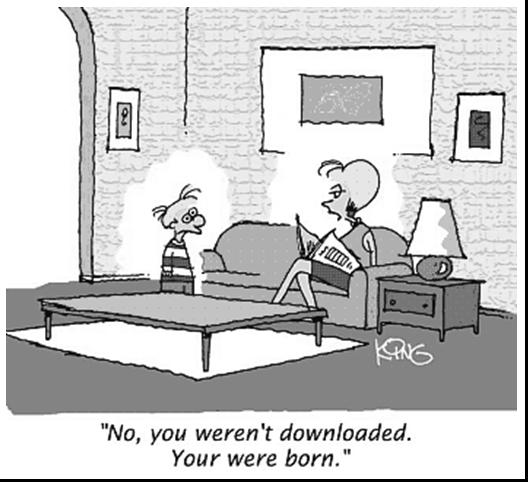
\includegraphics[width=16cm]{Figuras/fig1.jpg}
    }{
        \Fonte{Elaborado pelo Autor (2025)}
    }	
\end{figure}

Evite encerrar seções ou capítulos com figuras. Sempre adicione um texto explicativo após a figura para manter a fluidez do conteúdo.

\section{Inserindo Quadros}
\label{sec:quadros}

Quadros são utilizados para organizar informações de forma estruturada, especialmente quando se trata de dados qualitativos. O Quadro \ref{qua:exemplo-1} apresenta um exemplo de como inserir quadros no texto.

\begin{quadro}[h!]	
    \centering
    \Caption{\label{qua:exemplo-1} Exemplo de quadro com dados qualitativos}		
    \IFCEqua{}{
        \begin{tabular}{|c|c|l|l|}
            \hline
            Quisque & pharetra & tempus & vulputate \\
            \hline
            E1 & Complete coverage by a single transcript & Both  & Complete\\
            \hline
            E2 & Complete coverage by more than & Both splice sites & Complete\\
            \hline
            E3 & Partial coverage & Both splice sites & Both \\				
            \hline
        \end{tabular}
    }{
        \Fonte{Elaborado pelo autor.}
    }
\end{quadro}

\section{Inserindo Tabelas}
\label{sec:tabelas}

Tabelas são utilizadas para apresentar dados quantitativos organizadamente. A Tabela \ref{tab:exemplo-1} ilustra um exemplo de tabela alinhada. Ao inserir tabelas, siga as seguintes recomendações:

\begin{itemize}
    \item O título deve descrever o conteúdo da tabela de concisamente.
    \item Utilize linhas horizontais para separar os cabeçalhos dos dados. Evite o uso excessivo de linhas verticais.
    \item Sempre indique a fonte dos dados e inclua notas explicativas, se necessário.
\end{itemize}

\begin{table}[!h]
    \captionsetup{width=7cm} % Ajuste a largura do título para corresponder à tabela
    \Caption{\label{tab:exemplo-1} Exemplo de tabela com dados alinhados}
    \IBGEtab{}{%
        \begin{tabular}{ccc}
            \toprule
            Nome & Nascimento & Documento \\
            \midrule \midrule
            Maria da Silva & 11/11/1111 & 111.111.111-11 \\
            Maria da Silva & 11/11/1111 & 111.111.111-11 \\
            Maria da Silva & 11/11/1111 & 111.111.111-11 \\
            \bottomrule
        \end{tabular}%
    }{%
        \Fonte{O autor.}%
        \Nota{Esta é uma nota, que diz que os dados são baseados na regressão linear.}%
        \Nota[Anotações]{Uma anotação adicional, seguida de várias outras.}%
    }
\end{table}

\subsection{Exemplo de Subseção}
\label{sec:ex_sec}

Esta subseção serve como exemplo de como estruturar o conteúdo de forma hierárquica. Utilize subseções para dividir tópicos complexos em partes menores e mais gerenciáveis.

\section{Usando Fórmulas Matemáticas}
\label{sec:formulas}

Fórmulas matemáticas são frequentemente utilizadas em trabalhos acadêmicos para expressar relações quantitativas. Para inserir símbolos matemáticos no texto, utilize cifrões (\$). Por exemplo, $\alpha$, $\beta$ e $\gamma$ são símbolos do alfabeto grego. Para equações enumeradas, utilize o ambiente \texttt{equation}, como mostrado na Equação \ref{eq:indices}:

\begin{equation}
    \label{eq:indices}
    k_{n+1} = n^2 + k_n^2 - k_{n-1}.
\end{equation}

Observe que a equação faz parte da frase e deve ser pontuada corretamente. Ao referenciar a Equação \ref{eq:indices} no texto, utilize a primeira letra maiúscula.

Abaixo estão exemplos de equações com frações, matrizes e sistemas:

\begin{equation}
    \label{eq:fracao}
    \begin{aligned}
        x = a_0 + \cfrac{1}{a_1 + \cfrac{1}{a_2 + \cfrac{1}{a_3 + \cfrac{1}{a_4}}}}
    \end{aligned}.
\end{equation}

\begin{equation}
    \label{eq:matriz}
    \begin{aligned}
        A_{m,n} =
        \begin{pmatrix}
            a_{1,1} & a_{1,2} & \cdots & a_{1,n} \\
            a_{2,1} & a_{2,2} & \cdots & a_{2,n} \\
            \vdots  & \vdots  & \ddots & \vdots  \\
            a_{m,1} & a_{m,2} & \cdots & a_{m,n}
        \end{pmatrix}
    \end{aligned}.
\end{equation}

\begin{equation}
    \label{eq:sistema}
    \begin{aligned}
        f(n) = \left\{ 
        \begin{array}{l l}
            n/2 & \quad \text{se $n$ é par} \\
            -(n+1)/2 & \quad \text{se $n$ é ímpar}
        \end{array} \right.
    \end{aligned}.
\end{equation}

\vspace{0.5cm}

\begingroup
\let\clearpage\relax
\chapter{METODOLOGIA}\label{sec:metodologia}
\endgroup


A metodologia descreve os procedimentos e técnicas utilizados para conduzir a pesquisa. Esta seção deve apresentar, de forma clara e detalhada, os métodos adotados, os instrumentos de coleta de dados, a população ou amostra estudada, e as técnicas de análise. A escolha da metodologia deve ser justificada, demonstrando sua adequação aos objetivos da pesquisa.

\section{Tipo de Pesquisa}
\label{sec:tipo_pesquisa}

Este trabalho adota uma abordagem [descreva o tipo de pesquisa, por exemplo: quantitativa, qualitativa ou mista]. A pesquisa [quantitativa/qualitativa/mista] foi escolhida porque [justifique brevemente a escolha]. Para \citeonline{lamport1986latex}, esse tipo de abordagem é adequado para [explique por que é adequado].

\section{Procedimentos Metodológicos}
\label{sec:procedimentos}

Os procedimentos metodológicos foram divididos em etapas principais, conforme descrito a seguir:

\begin{itemize}
    \item \textbf{Definição do problema} [Descreva como o problema de pesquisa foi definido].
    \item \textbf{Revisão da literatura} [Explique como foi realizada a revisão bibliográfica].
    \item \textbf{Coleta de dados} [Descreva os métodos e instrumentos utilizados para coletar dados].
    \item \textbf{Análise dos dados} [Explique as técnicas de análise utilizadas].
\end{itemize}

\section{População e Amostra}
\label{sec:populacao_amostra}

A população deste estudo consiste em [descreva a população estudada]. A amostra foi selecionada por meio de [descreva o método de amostragem, por exemplo: amostragem aleatória simples, estratificada, etc.], totalizando [número de participantes ou unidades de análise]. A escolha desse método de amostragem justifica-se por [explique a justificativa].

\section{Instrumentos de Coleta de Dados}
\label{sec:instrumentos}

Para a coleta de dados, foram utilizados os seguintes instrumentos:

\begin{itemize}
    \item \textbf{Instrumento 1} [Descreva o instrumento e sua aplicação].
    \item \textbf{Instrumento 2} [Descreva o instrumento e sua aplicação].
    \item \textbf{Instrumento 3} [Descreva o instrumento e sua aplicação].
\end{itemize}

Cada instrumento foi escolhido com base em [justifique a escolha dos instrumentos]. Para garantir a validade e confiabilidade dos dados, [descreva as medidas adotadas, como pré-testes ou validação por especialistas].

\section{Técnicas de Análise de Dados}
\label{sec:analise_dados}

Os dados coletados foram analisados por meio das seguintes técnicas:

\begin{itemize}
    \item \textbf{Técnica 1}Utilizou-se o software [nome do software], que permite [explique brevemente as funcionalidades do software].
    \item \textbf{Técnica 2} Adotou-se [descreva a técnica e sua aplicação].
\end{itemize}

\section{Limitações da Pesquisa}
\label{sec:limitacoes}

Este estudo apresenta algumas limitações, tais como:

\begin{itemize}
    \item \textbf{Limitação 1} [Explique como isso pode afetar os resultados].
    \item \textbf{Limitação 2} [Explique como isso pode afetar os resultados].
    \item \textbf{Limitação 3} [Explique como isso pode afetar os resultados].
\end{itemize}

Apesar dessas limitações, acredita-se que os resultados obtidos são válidos e relevantes para [contexto da pesquisa].

\section{Considerações Éticas}
\label{sec:etica}

Este estudo foi conduzido em conformidade com as diretrizes éticas para pesquisas envolvendo [descreva o tipo de participação, por exemplo: seres humanos, animais, etc.]. O projeto foi aprovado pelo Comitê de Ética em Pesquisa da [instituição], sob o número de protocolo [número do protocolo]. Todos os participantes assinaram um Termo de Consentimento Livre e Esclarecido (TCLE), garantindo o sigilo e a confidencialidade das informações coletadas.

\vspace{0.5cm}
\par
\begingroup
\let\clearpage\relax
\chapter{RESULTADOS}
\label{sec:resultados}
\endgroup

São apresentados os resultados temporais e municipais dos registros classificados como dengue no Ceará entre 2016 e 2025, incluindo taxas populacionais, recorrência e distribuição espacial nos 184 municípios.

\section{Distribuição temporal dos registros}
\label{sec:resultados_temporais}

A série temporal reuniu 215.251 registros. Os maiores totais anuais ocorreram em 2016 (41.894) e 2022 (39.940), enquanto 2018 apresentou 3.995 registros, o menor valor entre 2016 e 2024. O total de 2025 requer cautela, pois sua completude não foi confirmada.

Entre março e junho, concentraram-se 141.020 registros (65,5\% do total). Maio acumulou 44.018 registros, com média anual de 4.401,8. Em todos os anos, os maiores totais mensais ocorreram entre abril e junho; o pico da série foi registrado em maio de 2022 (10.601). Essa concentração caracteriza sazonalidade descritiva, sem estabelecer associação causal com o clima.

\section{Distribuição municipal por números absolutos}
\label{sec:resultados_municipais}

A base municipal reuniu 215.243 registros válidos nos 184 municípios. Fortaleza concentrou 90.035 registros (41,83\%), seguida por Brejo Santo, com 7.249 (3,37\%), e Caucaia, com 6.155 (2,86\%). A Figura \ref{fig:top10_municipios} apresenta os dez maiores totais acumulados; essas contagens não consideram diferenças populacionais.

\begin{figure}[!htbp]
    \centering
    \captionsetup{width=16cm}
    \Caption{\label{fig:top10_municipios} Dez municípios com maiores totais acumulados de registros classificados de dengue no Ceará, 2016--2025}
    \IFCEfig{}{
        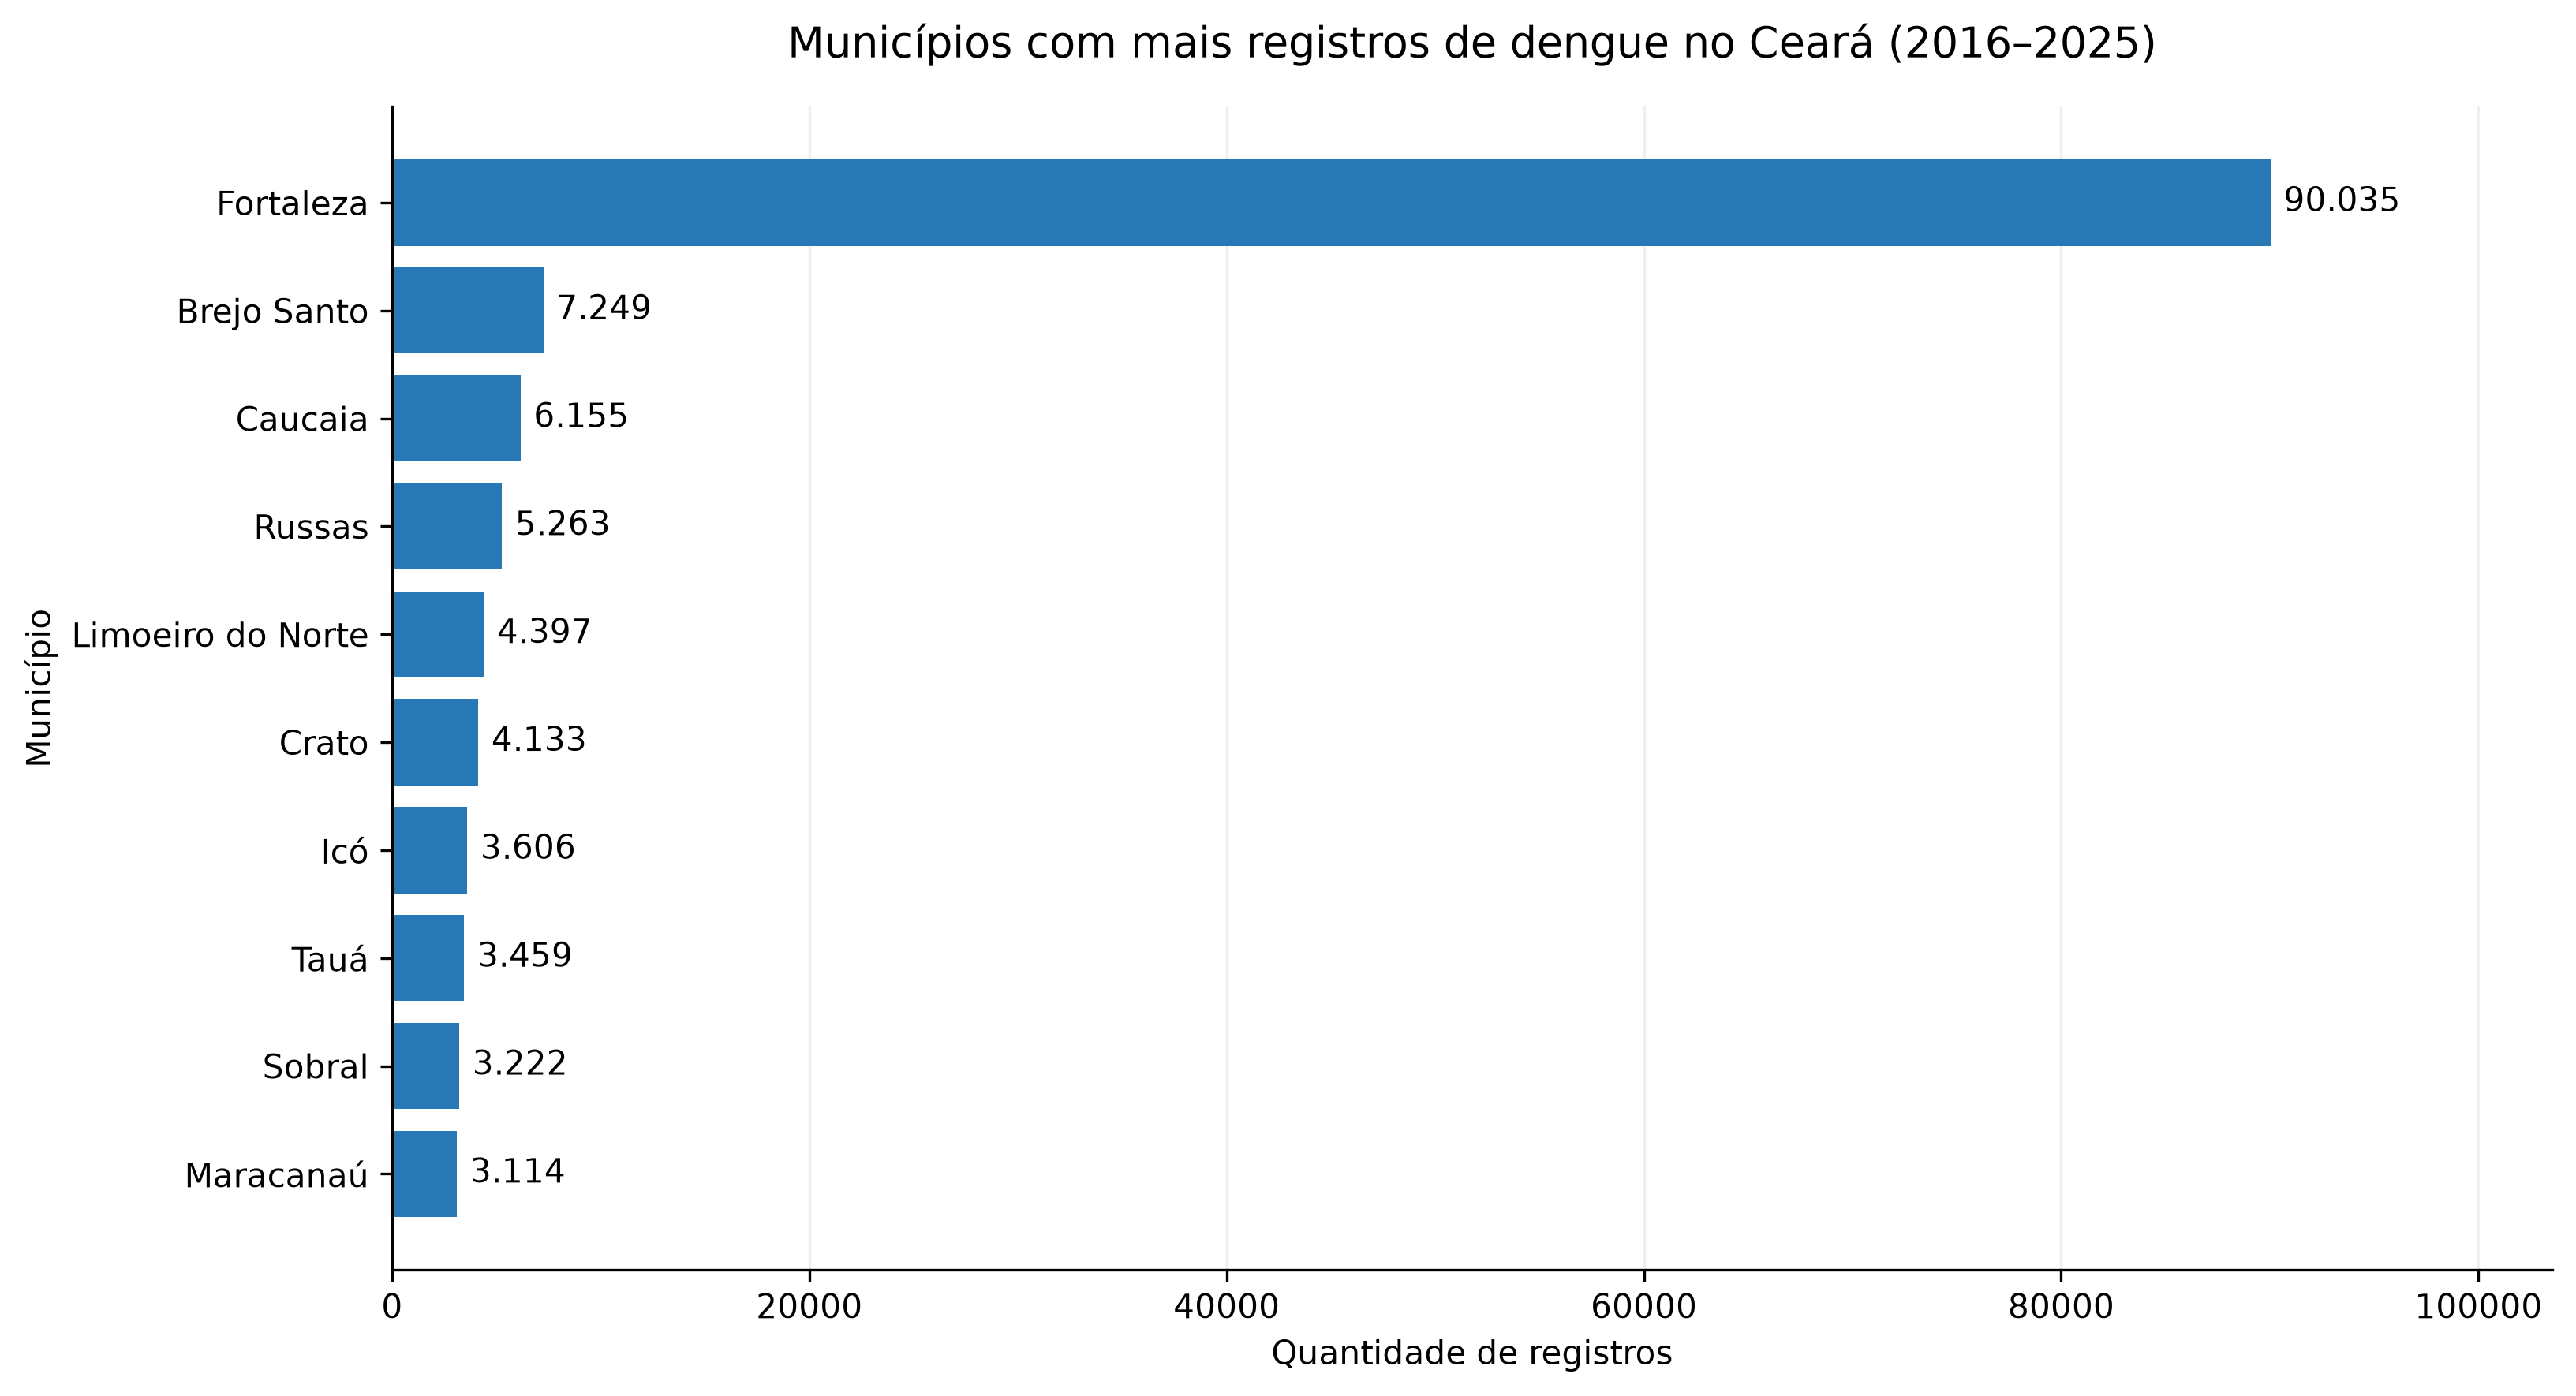
\includegraphics[width=\textwidth]{Figuras/top10_municipios_2016_2025.png}
    }{
        \Fonte{Elaborado pelo autor a partir de dados do Ministério da Saúde.}
    }
\end{figure}
\FloatBarrier

\section{Taxas anuais agregadas do Ceará}
\label{sec:resultados_taxas_estaduais}

A Tabela \ref{tab:taxas_estaduais} apresenta as taxas anuais calculadas com registros de municípios válidos e respectivas populações. As maiores ocorreram em 2016 (467,38) e 2022 (454,10), contrastando com 2018 (44,02 registros por 100 mil habitantes). Trata-se de indicadores desta pesquisa, não de taxas oficiais de incidência.

\begin{table}[!htbp]
    \centering
    \caption{Registros municipais e taxas anuais por 100 mil habitantes no Ceará, 2016--2025}
    \label{tab:taxas_estaduais}
    \small
    \begin{tabular}{rrrr}
        \toprule
        Ano & Registros & População & Taxa por 100 mil \\
        \midrule
        2016 & 41.894 & 8.963.663 & 467,38 \\
        2017 & 27.055 & 9.020.460 & 299,93 \\
        2018 & 3.995 & 9.075.649 & 44,02 \\
        2019 & 15.674 & 9.132.078 & 171,64 \\
        2020 & 21.451 & 9.187.103 & 233,49 \\
        2021 & 33.841 & 9.240.580 & 366,22 \\
        2022 & 39.938 & 8.794.957 & 454,10 \\
        2023 & 14.220 & 8.794.957 & 161,68 \\
        2024 & 12.127 & 9.233.656 & 131,33 \\
        2025 & 5.048 & 9.268.836 & 54,46 \\
        \bottomrule
    \end{tabular}

    \vspace{0.2cm}
    \begin{minipage}{\textwidth}
        \footnotesize
        Fonte: elaboração própria a partir de dados do Ministério da Saúde e do IBGE.

        Nota: os totais municipais excluem oito registros sem município cearense válido. A população de 2023 utiliza referência baseada no Censo de 2022.
    \end{minipage}
\end{table}
\FloatBarrier

\section{Evolução das taxas de Brejo Santo e do Ceará}
\label{sec:brejo_ceara}

Conforme a Figura \ref{fig:brejo_ceara}, Brejo Santo superou a taxa estadual em oito dos dez anos, exceto em 2016 e 2021. Suas taxas em 2017, 2023 e 2024 foram, respectivamente, de 2.877,33, 3.491,88 e 4.425,60 registros por 100 mil habitantes, equivalentes a cerca de 9,59, 21,60 e 33,70 vezes as taxas estaduais. A comparação não identifica as causas dessas diferenças.

\begin{figure}[!htbp]
    \centering
    \captionsetup{width=12cm}
    \Caption{\label{fig:brejo_ceara} Evolução das taxas de registros classificados de dengue em Brejo Santo e no Ceará, 2016--2025}
    \IFCEfig{}{
        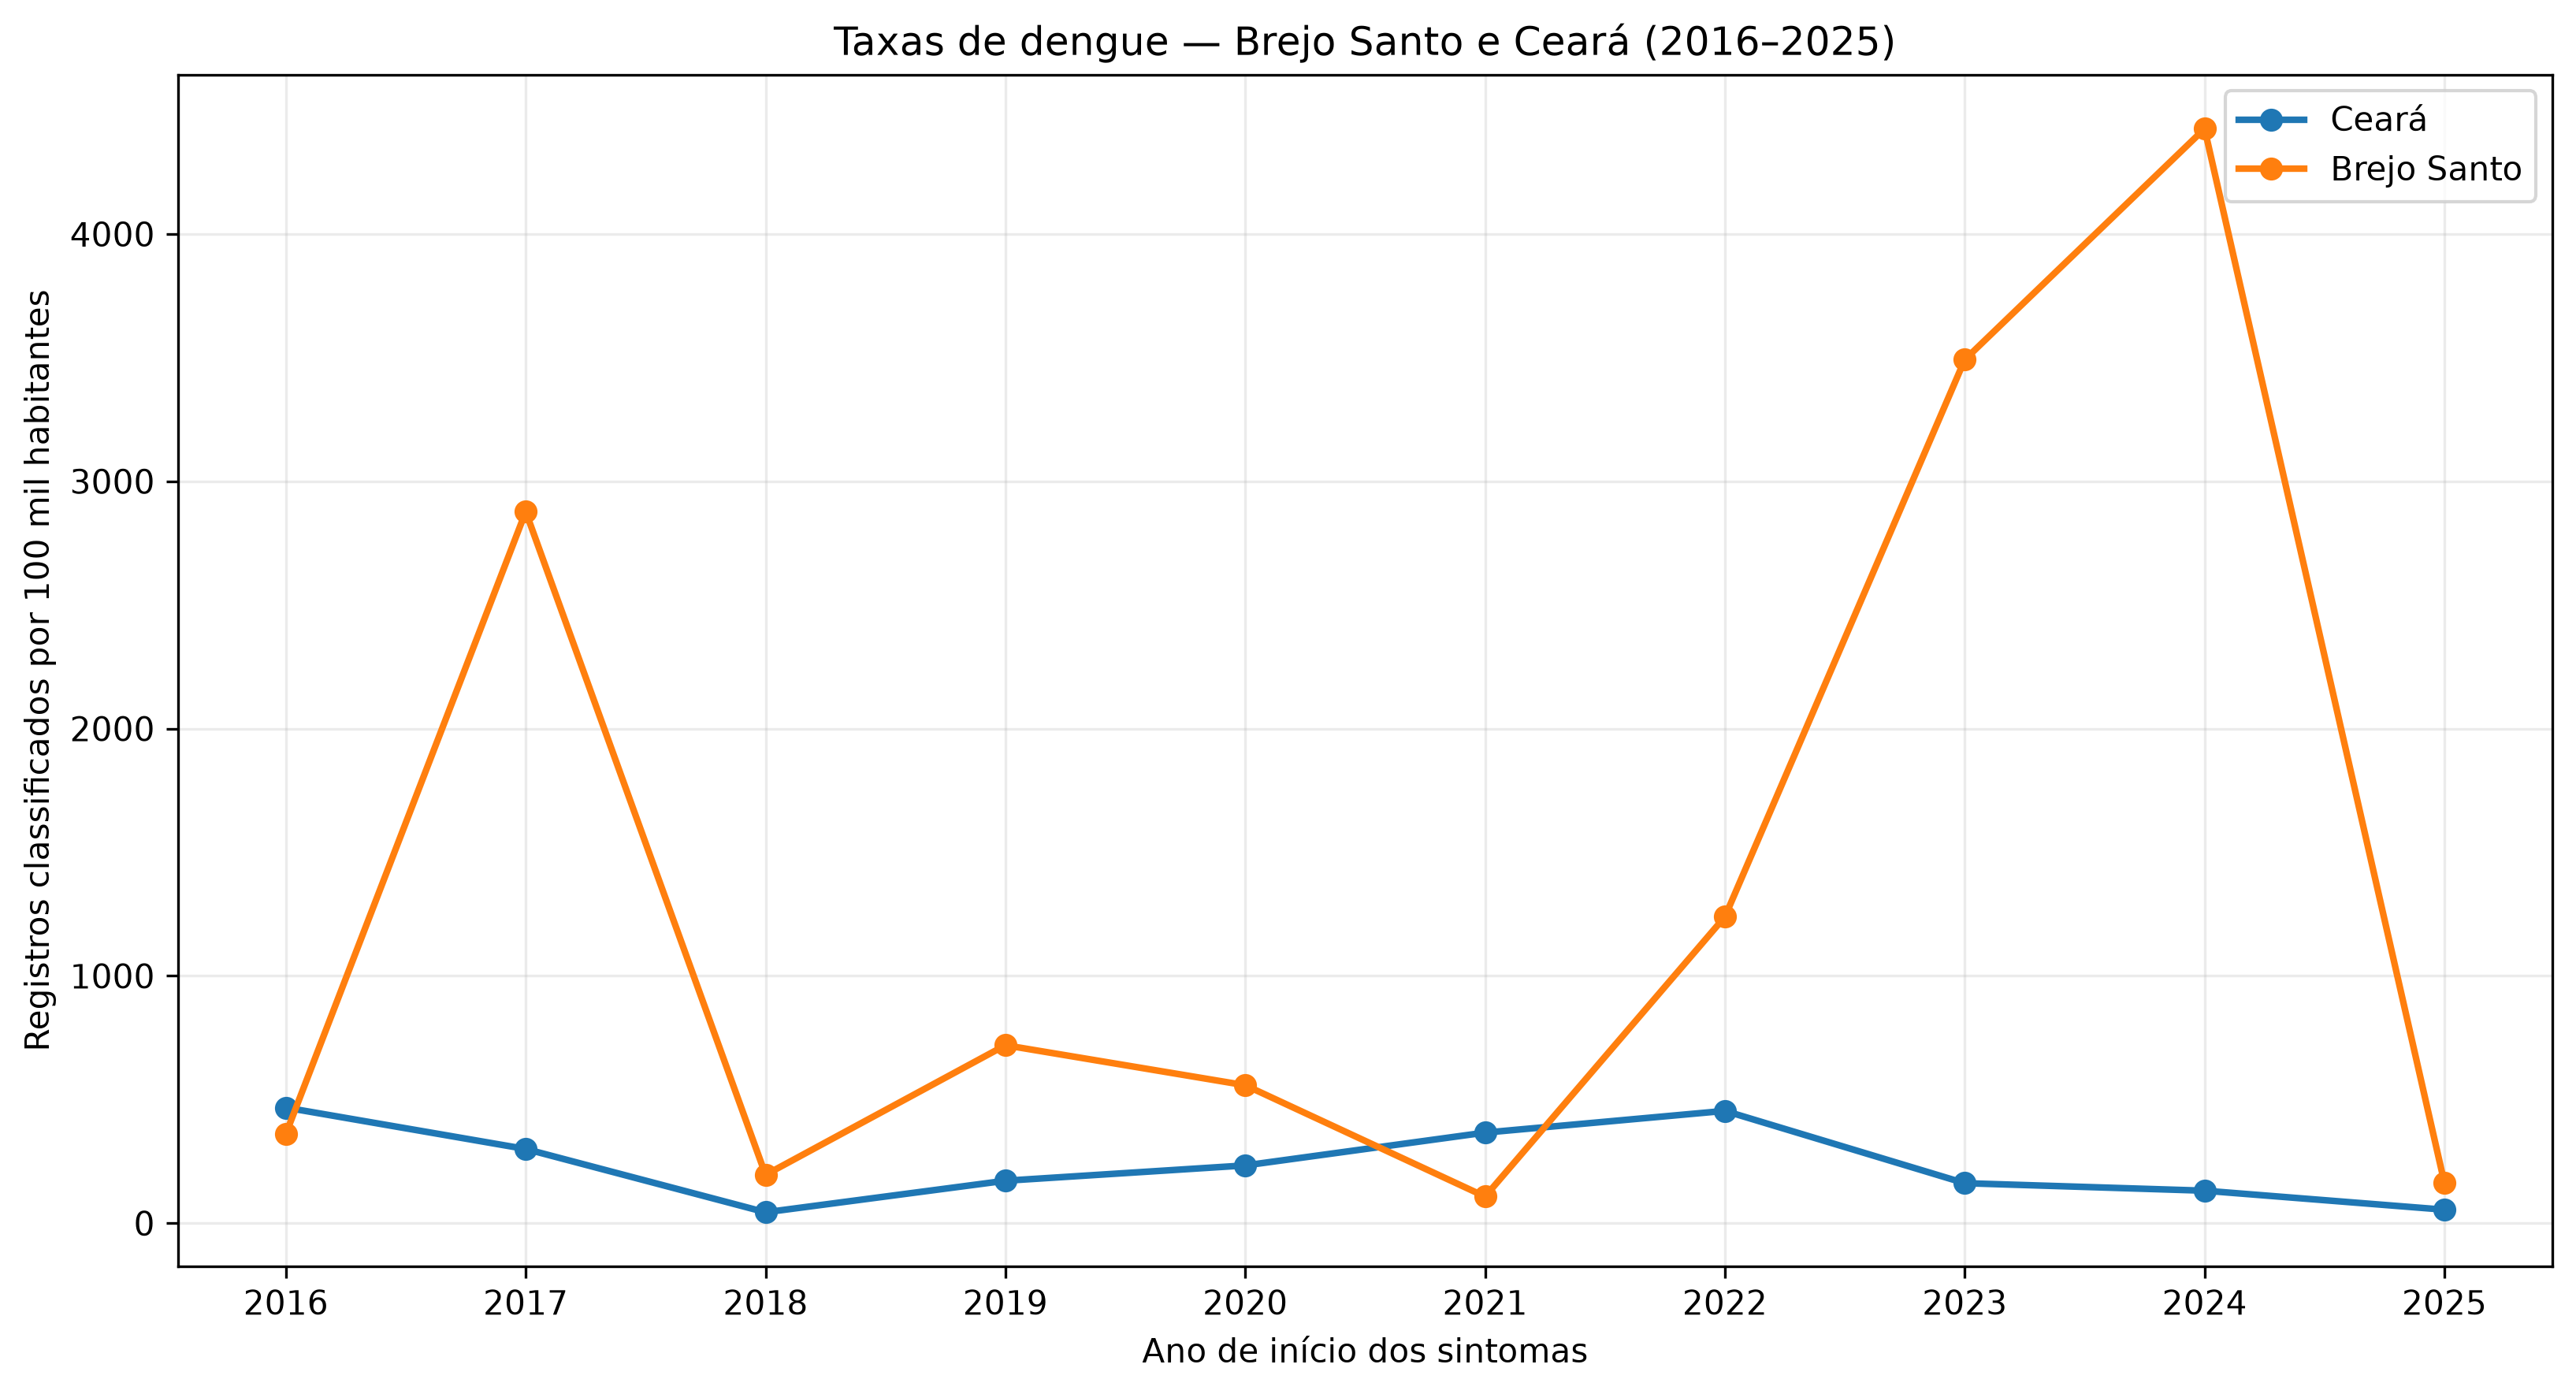
\includegraphics[width=\textwidth,height=\textheight,keepaspectratio]{Figuras/comparativo_brejo_ceara_2016_2025.png}
    }{
        \Fonte{Elaborado pelo autor a partir de dados do Ministério da Saúde e do IBGE.}
    }
\end{figure}
\FloatBarrier

\section{Recorrência de taxas municipais superiores à estadual}
\label{sec:recorrencia_municipal}

Brejo Santo, Quixeré, Tabuleiro do Norte e Fortaleza apresentaram taxas superiores à estadual em oito dos dez anos; Penaforte, Icapuí, Jaguaribara e Limoeiro do Norte, em sete. A Figura \ref{fig:heatmap_municipal} compara as taxas anuais dos 15 municípios selecionados por maior recorrência, evidenciando variações entre municípios e anos. A recorrência expressa posição relativa à taxa estadual, não taxas necessariamente elevadas em termos absolutos.

\begin{figure}[!htbp]
    \centering
    \captionsetup{width=16cm}
    \Caption{\label{fig:heatmap_municipal} Taxas anuais dos 15 municípios selecionados por maior recorrência acima da taxa estadual, 2016--2025}
    \IFCEfig{}{
        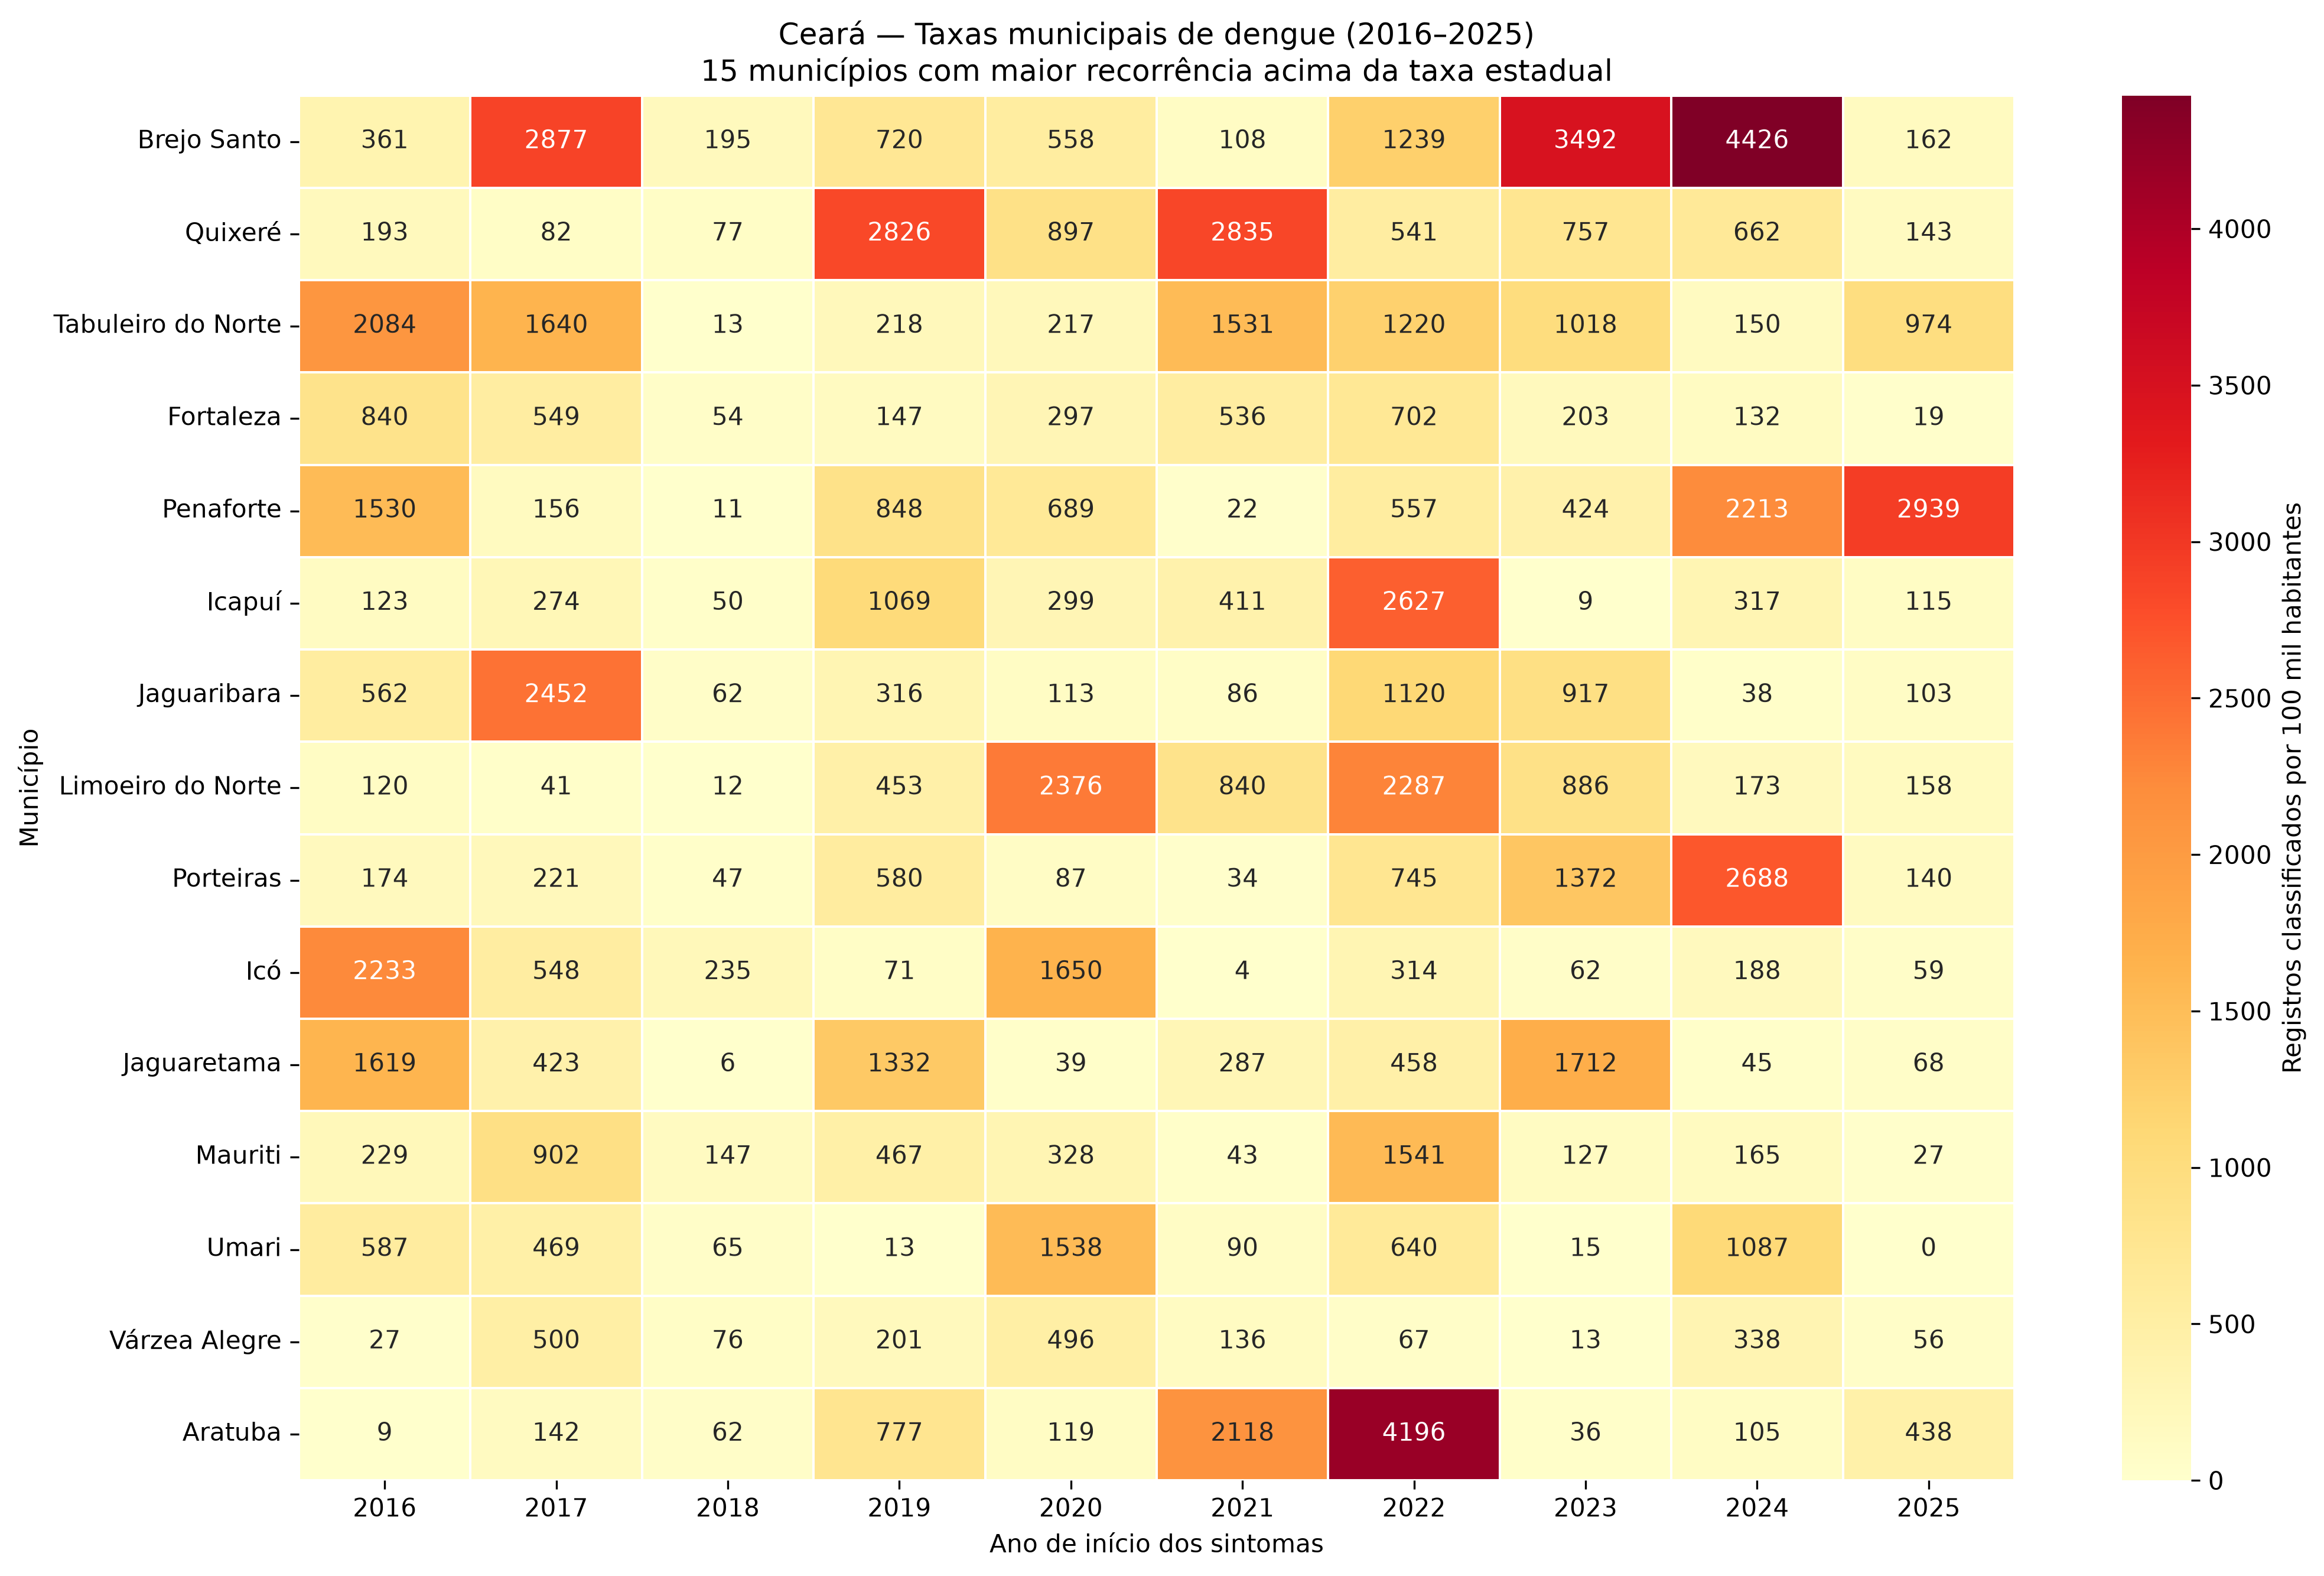
\includegraphics[width=\textwidth]{Figuras/heatmap_taxas_municipais.png}
    }{
        \Fonte{Elaborado pelo autor a partir de dados do Ministério da Saúde e do IBGE.}
    }
\end{figure}
\FloatBarrier

\section{Distribuição espacial das taxas municipais}
\label{sec:resultados_espaciais}

Os mapas históricos (Figura \ref{fig:mapas_historicos}) mostram variação espacial das taxas nos 184 municípios. O número de municípios com taxas superiores a 700 registros por 100 mil habitantes foi de 27 em 2022, dois em 2018, 22 em 2016 e em 2021 e nove em 2024. Em 2016, 11 municípios superaram 1.500 registros por 100 mil habitantes, o maior total nessa faixa na série.

As classes dos mapas são descritivas e constantes durante a série, permitindo comparação visual sem comprovar agrupamentos espaciais estatisticamente significativos.

\begin{figure}[!htbp]
    \centering
    \captionsetup{width=16cm}
    \Caption{\label{fig:mapas_historicos} Distribuição municipal das taxas de registros classificados de dengue no Ceará, 2016--2025}
    \IFCEfig{}{
        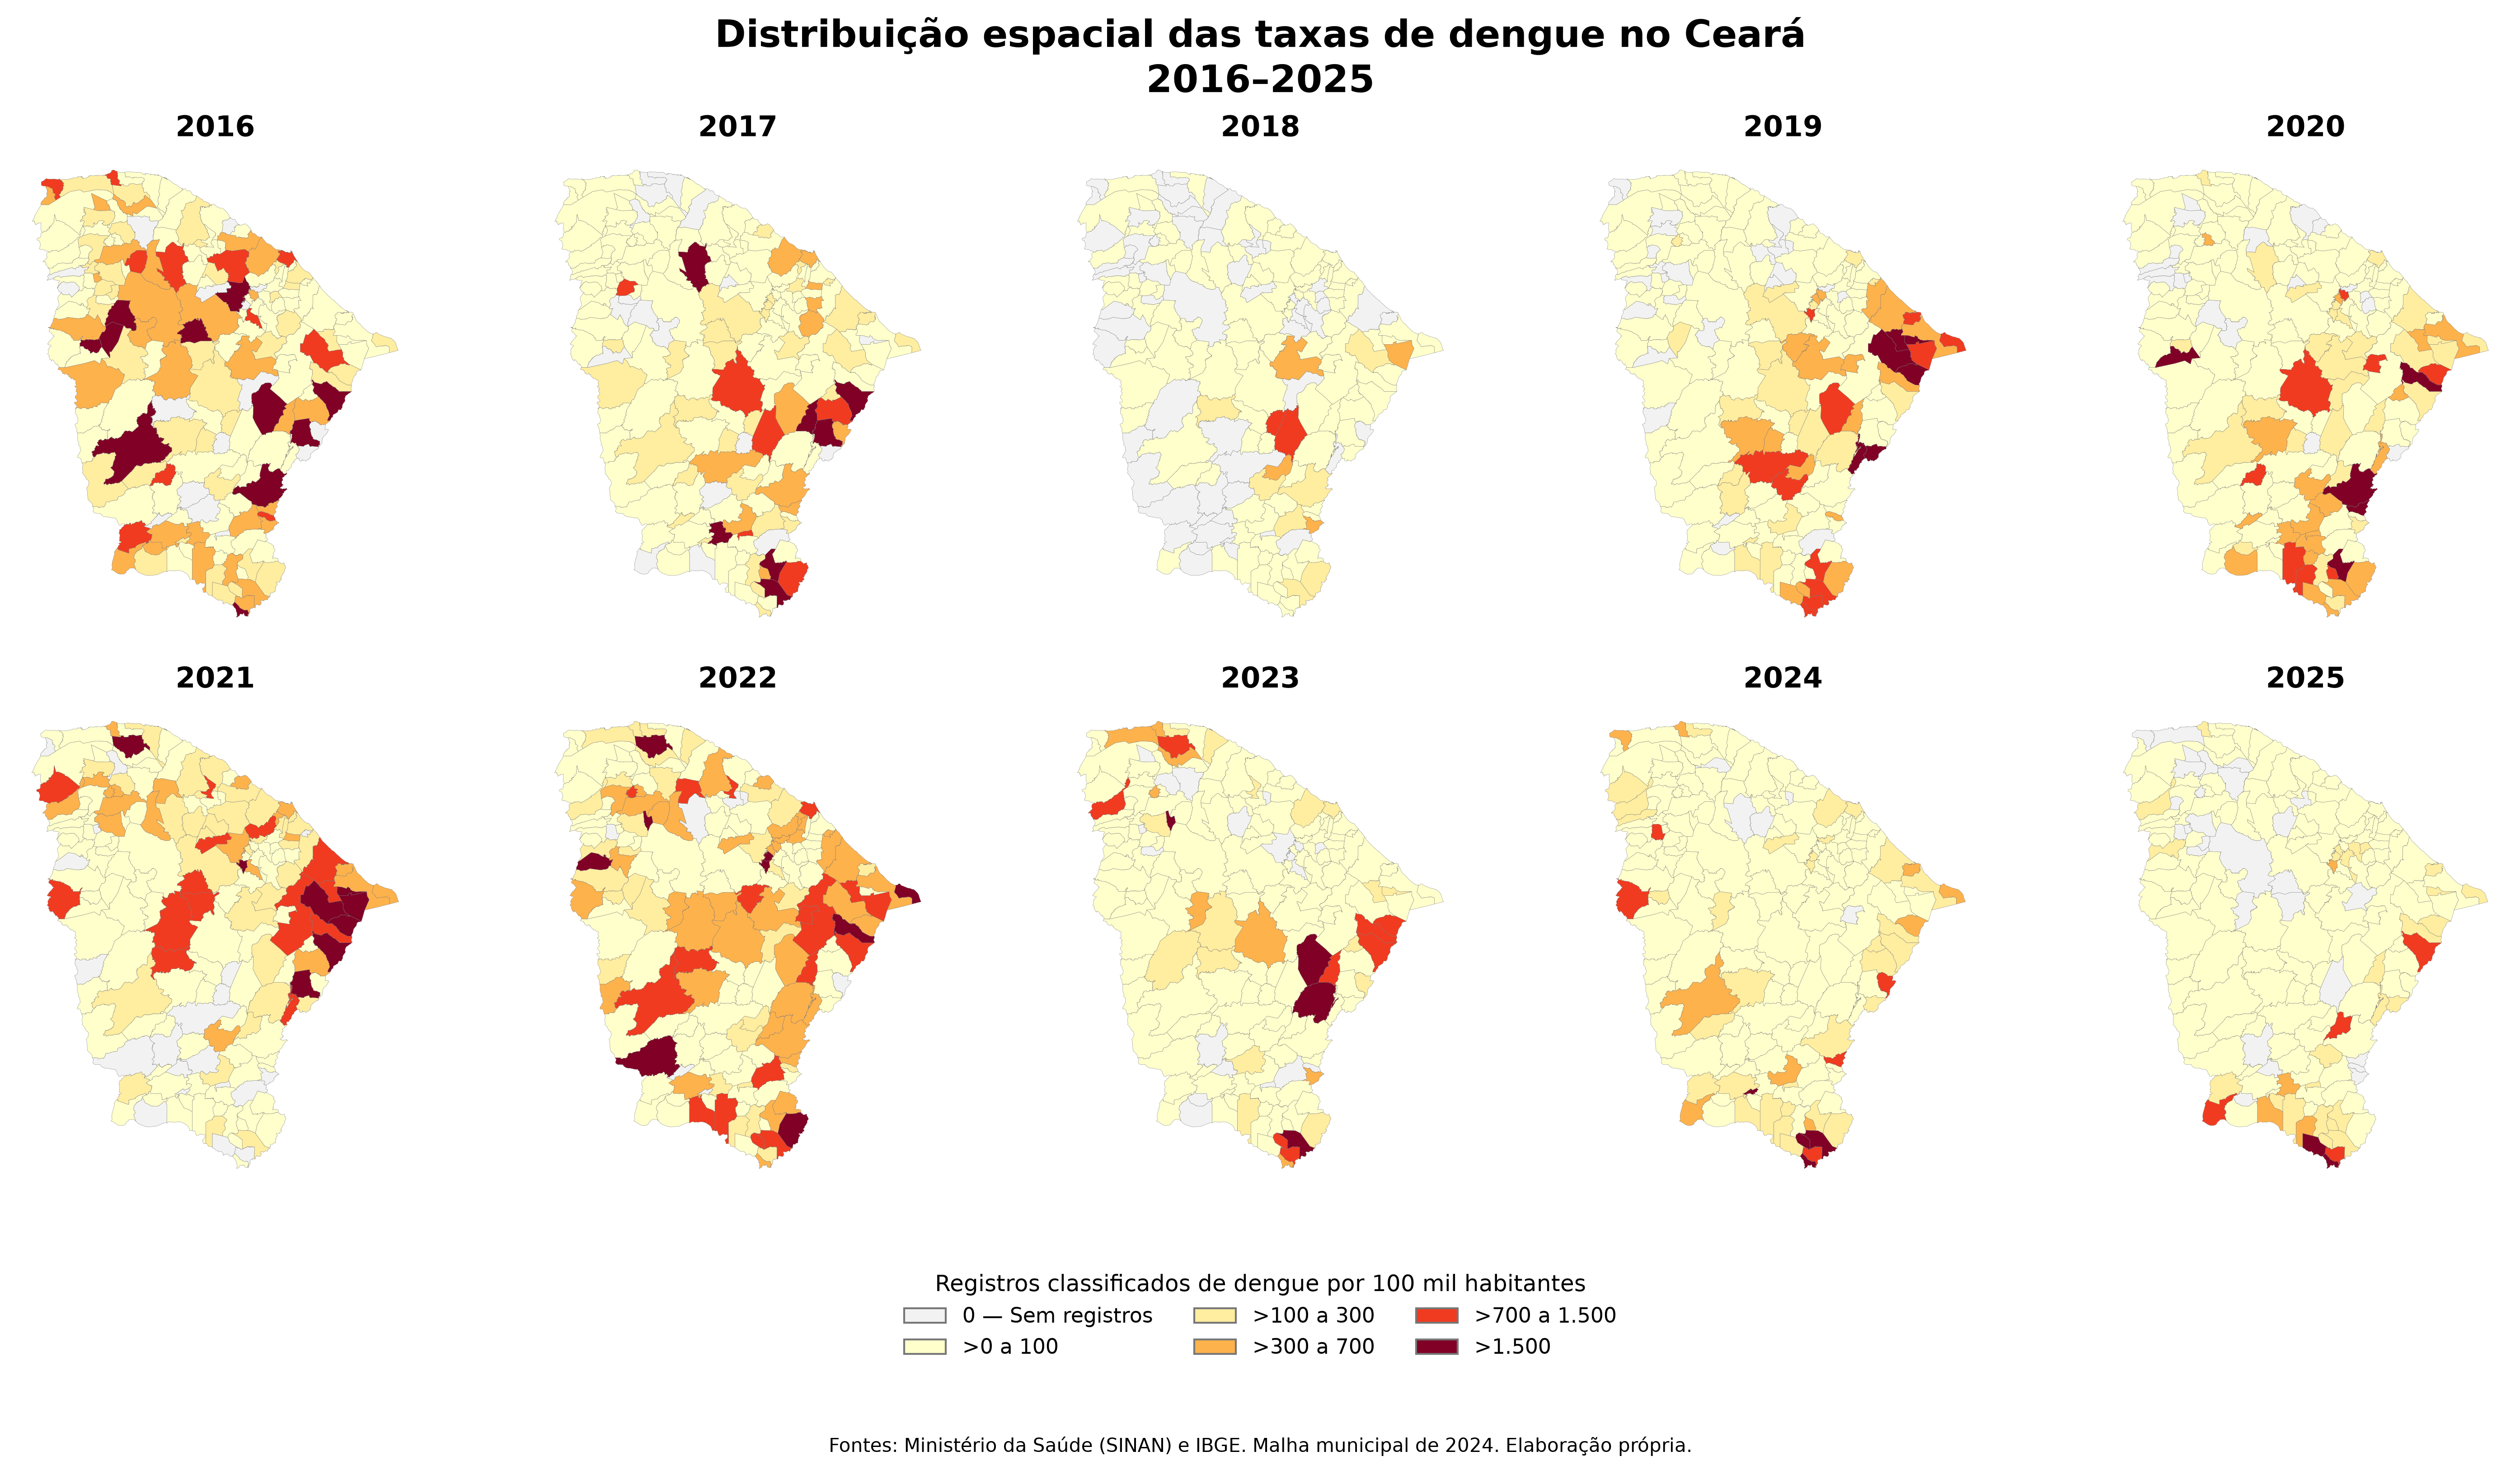
\includegraphics[width=\textwidth]{Figuras/mapas_historicos_dengue_2016_2025.png}
    }{
        \Fonte{Elaborado pelo autor a partir de dados do Ministério da Saúde e do IBGE.}
    }
\end{figure}
\FloatBarrier

\section{Limitações na interpretação dos resultados}
\label{sec:limitacoes_resultados}

A interpretação depende da qualidade das classificações, de possíveis duplicidades e das fontes populacionais. A exclusão dos 62 registros com intervalo superior a 365 dias pode afetar as agregações; a referência populacional de 2023 baseia-se no Censo de 2022 e a completude de 2025 não foi confirmada. A malha municipal de 2024 foi aplicada aos dez anos. Assim, contagens e taxas não equivalem necessariamente a casos únicos ou à incidência oficial, e os padrões observados não demonstram causalidade nem dependência espacial significativa.

\vspace{0.5cm}

\begingroup
\let\clearpage\relax
\chapter{conclusão}\label{sec:matemet}
\endgroup

\vspace{0,5cm}

Parte final do texto na qual se apresentam as conclusões apoiadas no desenvolvimento do assunto. É a recapitulação sintética dos resultados obtidos. Pode apresentar recomendações e sugestões para pesquisas futuras.

\bibliography{03-pos-textual/referencias}

\end{document}